\section{eo\-Select\-Factory$<$ EOT $>$ Class Template Reference}
\label{classeo_select_factory}\index{eoSelectFactory@{eoSelectFactory}}
{\bf EO}{\rm (p.\,\pageref{class_e_o})} Factory.An instance of the factory class to create selectors, that is, {\bf eo\-Select}{\rm (p.\,\pageref{classeo_select})} objects.  


{\tt \#include $<$eo\-Select\-Factory.h$>$}

Inheritance diagram for eo\-Select\-Factory$<$ EOT $>$::\begin{figure}[H]
\begin{center}
\leavevmode
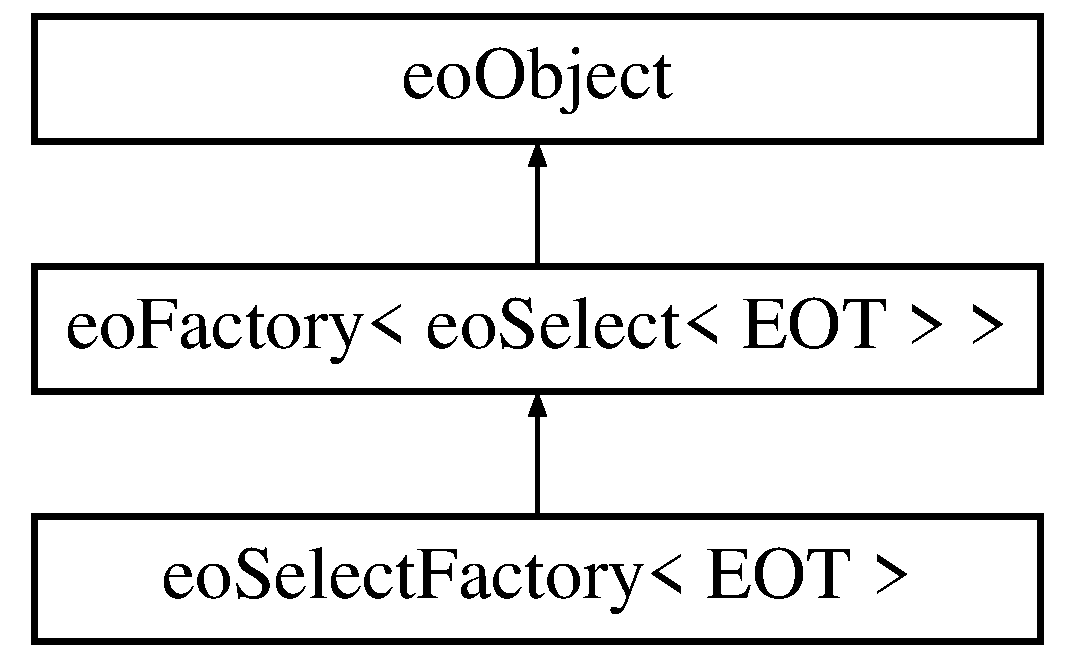
\includegraphics[height=3cm]{classeo_select_factory}
\end{center}
\end{figure}
\subsection*{Public Member Functions}
\begin{CompactItemize}
\item 
virtual {\bf eo\-Select}$<$ {\bf EOT} $>$ $\ast$ {\bf make} (std::istream \&\_\-is)
\begin{CompactList}\small\item\em Another factory methods: creates an object from an std::istream, reading from it whatever is needed to create the object. \item\end{CompactList}\end{CompactItemize}
\begin{Indent}{\bf ctors and dtors}\par
\begin{CompactItemize}
\item 
{\bf eo\-Select\-Factory} ()\label{classeo_select_factory_z20_0}

\begin{CompactList}\small\item\em constructor \item\end{CompactList}\item 
virtual {\bf $\sim$eo\-Select\-Factory} ()\label{classeo_select_factory_z20_1}

\begin{CompactList}\small\item\em destructor \item\end{CompactList}\end{CompactItemize}
\end{Indent}
\begin{Indent}{\bf eo\-Object methods}\par
\begin{CompactItemize}
\item 
void {\bf print\-On} (std::ostream \&\_\-os) const \label{classeo_select_factory_z22_0}

\item 
void {\bf read\-From} (std::istream \&\_\-is)\label{classeo_select_factory_z22_1}

\end{CompactItemize}
\end{Indent}


\subsection{Detailed Description}
\subsubsection*{template$<$class EOT$>$ class eo\-Select\-Factory$<$ EOT $>$}

{\bf EO}{\rm (p.\,\pageref{class_e_o})} Factory.An instance of the factory class to create selectors, that is, {\bf eo\-Select}{\rm (p.\,\pageref{classeo_select})} objects. 

\begin{Desc}
\item[See also:]{\bf eo\-Select}{\rm (p.\,\pageref{classeo_select})} \end{Desc}




Definition at line 39 of file eo\-Select\-Factory.h.

\subsection{Member Function Documentation}
\index{eoSelectFactory@{eo\-Select\-Factory}!make@{make}}
\index{make@{make}!eoSelectFactory@{eo\-Select\-Factory}}
\subsubsection{\setlength{\rightskip}{0pt plus 5cm}template$<$class EOT$>$ virtual {\bf eo\-Select}$<${\bf EOT}$>$$\ast$ {\bf eo\-Select\-Factory}$<$ {\bf EOT} $>$::make (std::istream \& {\em \_\-is})\hspace{0.3cm}{\tt  [inline, virtual]}}\label{classeo_select_factory_a0}


Another factory methods: creates an object from an std::istream, reading from it whatever is needed to create the object. 

Usually, the format for the std::istream will be$\backslash$ object\-Type parameter1 parameter2 ... parametern$\backslash$

Implements {\bf eo\-Factory$<$ eo\-Select$<$ EOT $>$ $>$} {\rm (p.\,\pageref{classeo_factory_a0})}.

Definition at line 56 of file eo\-Select\-Factory.h.

The documentation for this class was generated from the following file:\begin{CompactItemize}
\item 
eo\-Select\-Factory.h\end{CompactItemize}
